% Operations Manual Chapter Title 
\infolevone{
\chapter[General Description]{General Description
\footnote{Authors: D. Higinbotham \email{doug@jlab.org} with many thanks to A.Saha$^{Deceased}$}}
\section{Introduction}
\label{sec:beam-intro}
}
% ESAD Section Title
\infoleveqnull{\section{Beamline}}

The control and measurement equipment along the Hall A beamline consists of 
various elements necessary to transport beam with the required specifications 
onto the reaction target and the dump and to simultaneously measure the 
properties of the beam relevant to the successful implementation of the 
physics program in Hall A.  

\infolevone{
The resolution and accuracy requirements in Hall 
A are such that special attention is paid to the following:
\begin{list}{\arabic{enumi}.~}{\usecounter{enumi}\setlength{\itemsep}{-0.15cm}}
  \item Determination of the incident beam energy;
  \item Control of the beam position, direction, emittance and stability;
  \item Determination of the beam current;
  \item Determination of the beam polarization.
\end{list}

A schematic of the Hall A line starting at the shield wall is
shown on Fig.~\ref{fig:Aline1},~\ref{fig:Aline2} and \ref{fig:Aline3}. 

\begin{figure}
\begin{center}
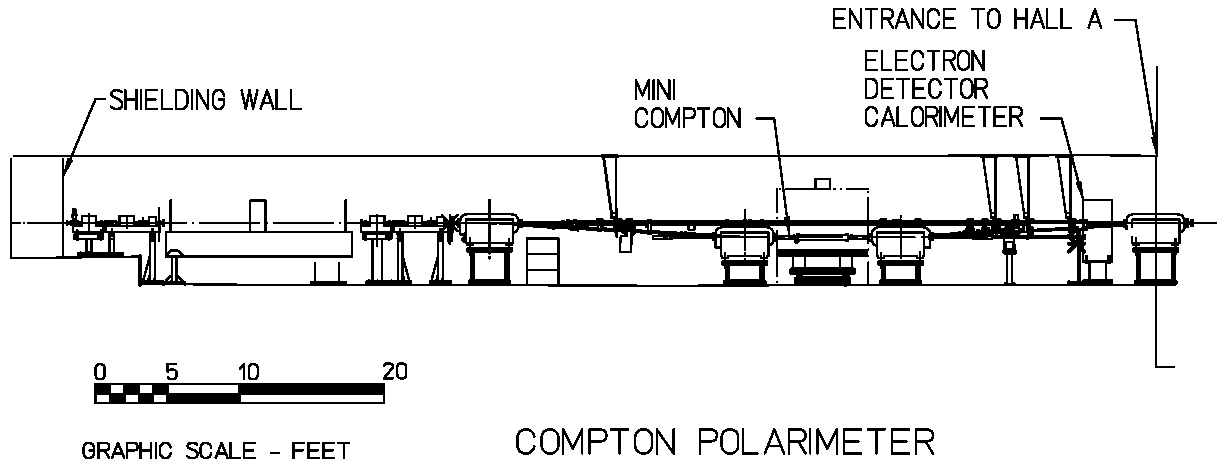
\includegraphics[angle=0,width=15cm]{compton_r}
\caption[Beamline: Hall A Beamline Overview]{Schematic of the Hall A beamline
starting at the shield wall to end of alcove.}
\label{fig:Aline1}
\end{center}
\end{figure}

\begin{figure}
\begin{center}
\includegraphics[angle=0,width=15cm]{aline}
\caption[Beamline: Hall A Beamline Overview]{Schematic of the Hall A beamline
from the end of the alcove to the target chamber.  This image has been updated
to show the new larger raster system as well as the new Moller magnets.}
\label{fig:Aline2}
\end{center}
\end{figure}

\begin{figure}
\begin{center}
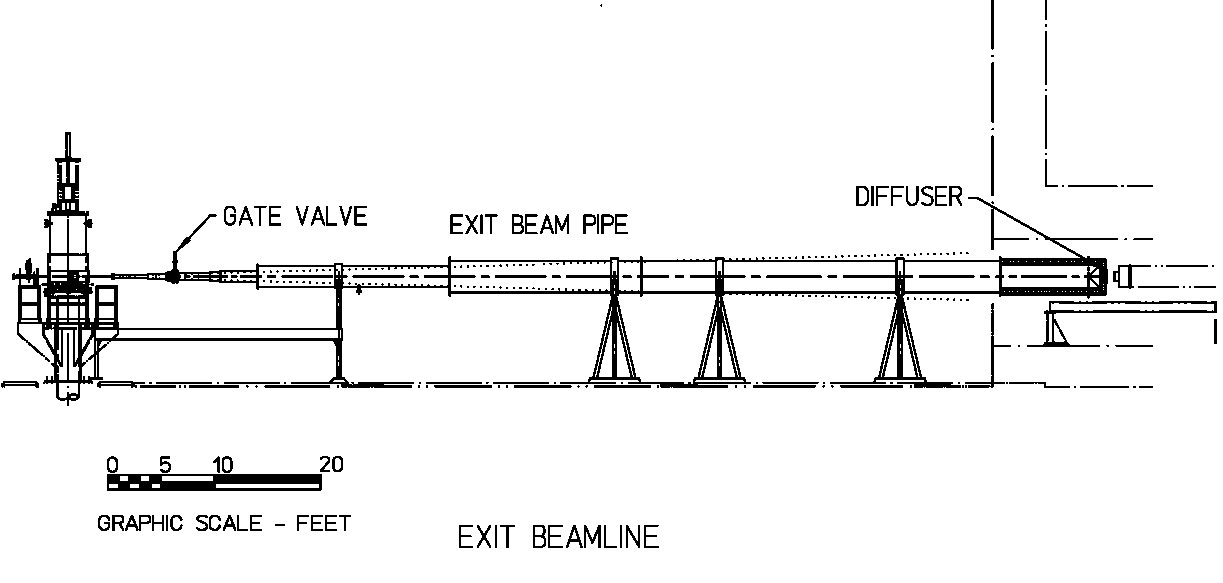
\includegraphics[angle=0,width=15cm]{dump_r}
\caption[Beamline: Hall A Beamline Overview]{Schematic of the Hall A beamline
from the target chamber to the dump diffuser.}
\label{fig:Aline3}
\end{center}
\end{figure}
}

\infolevtwo{
\subsection{The Beam Entrance Channel}

The beam entrance channel consists of 63.5 mm inner diameter stainless steel 
tubing connected with conflat flanges. Through magnets the inner diameter of the 
tubing is restricted to 25.4 mm. 
%%NOTE: 'tab:beam_tab1' is in beamline/tables.tex, but this is not included anywhere
%Sections are isolated by vacuum valves and these are listed in Table~\ref{tab:beam_tab1}. 
Each section has a roughing port and is pumped with an ion pump. 
The pressure is about 10$^{-6}$ Torr. There are several sections along the 
beamline where users interface their equipment. Their individual systems 
are tested leak tight (to $ \le 10^{-9}$ Atm cm$^3$/sec).

\subsection{The Beam Optics Channel}

These consist of dipoles, quadrupoles, sextupoles, and 
beam correctors with their 
standard girders and stands. Starting from the beam switch yard, there are 
eight dipoles in the arc section which (along with five  other smaller beam 
deflectors) bend the beam 37.5 degrees into the hall. Each dipole has a 
quadrupole and a pair of steering magnets (correctors) associated with it. 
After the shield wall at the entrance to the tunnel into the hall the beam is 
essentially undeflected onto the target and into the dump.  

The beamline optics elements are designed to deliver 
various optical tunes of the beam on to the physics target as well as 
simultaneously deliver various optical tunes at other locations along the 
beamline. These requirements are listed in Tables \ref{beam_tab3} and \ref{beam_tab4}. 
For the basic beamline we 
are able to deliver beam onto the hall A target in the achromatic
mode. 
 
\begin{table}[hp]
\begin{center}
\begin{tabular}{|c|c|c|c|c|} \hline
{\bf Mode} & {\bf Spot Size} & {\bf Dispersion} & {\bf Position} & {\bf
Size} \\
& {\bf 4$\cdot\sigma_{x,y}$} & {\bf $\eta$} & {\bf Stability} & {\bf
Stability} \\ \hline
Achromat & 140$\mu$m & 0 & 50$\mu$m & 50$\mu$m \\ \hline
Dispersive & $\propto \eta\delta$ & 4m to 12m & 50$\mu$m & 50$\mu$m \\
\hline
Defocussed & 0 to 3mm & 0 & $\pm$10\% & $\pm$10\% \\ \hline
\end{tabular}
\end{center}
\caption[Beamline: Optics Requirements Target]{ Line A Optics and Beam Requirements at Target}
\label{beam_tab3}
\end{table}

\newcounter{footnotetmp1}
\setcounter{footnotetmp1}{\value{footnote}}
\stepcounter{footnotetmp1}
\newcounter{footnotetmp2}
\setcounter{footnotetmp2}{\value{footnotetmp1}}
\stepcounter{footnotetmp2}
\begin{table}[h]
\begin{center}
\begin{tabular}{|c|c|c|c|c|} \hline
{\bf Mode} & {\bf Spot Size} & {\bf Dispersion} & {\bf Position} & {\bf Size} \\
& {\bf $4\cdot{}\sigma_{x,y}$} & {\bf $\eta$} & {\bf Stability} & {\bf Stability} \\ \hline
Energy-eP  {\color{red}\footnotemark[\arabic{footnotetmp1}]} & $>$100$\mu$m & 0 & 50$\mu$m & 50$\mu$m \\ \hline
Moller Pol.{\color{red}\footnotemark[\arabic{footnotetmp1}]} & $>$250$\mu$m & 0 & 50$\mu$m & 50$\mu$m \\ \hline
Compton Pol.  & $>$80$\mu$m & 0 & 50$\mu$m & 50$\mu$m \\ \hline
Energy-arc {\color{red}\footnotemark[\arabic{footnotetmp1}]~\footnotemark[\arabic{footnotetmp2}]} && 15m & 50$\mu$m & 50$\mu$m \\ \hline
\end{tabular}
\end{center}
\caption[Beamline: Optics Requirements Other]{ Line A Optics and
         Beam Requirements at Other Locations.
}
\label{beam_tab4}
\end{table}
\addtocounter{footnote}{2}
\footnotetext[\value{footnotetmp1}]{Destructive measurements.}
\footnotetext[\value{footnotetmp2}]{Build dispersion in arc section with all 
             magnetic elements except dipoles turned off.}

Build dispersion in arc section with all magnetic elements except
dipoles turned off.

\subsection{Beam Diagnostic Elements}

These consist of beam position monitors (BPMs), beam current monitors,  wire 
scanners (superharps) and beam loss monitors. 
The wire scanners are fabricated by Saclay (French 
collaboration) and four have been installed along the beamline, two before 
the arc section and two after the arc section. They are essential for the 
beam energy determination by the arc method. Another two wire scanners are
installed on the bench just before the target to determine the beam 
position and direction of the beam at the target point with high precision 
and also measure the emittance of the incident beam. They are also used to  
absolutely calibrate the two associated beam position monitors located  in 
front of the target. 

To determine the position and the direction of the beam on the experimental 
target point, two Beam Position Monitors (BPMs) are located at distances 7.524 m 
(IPM1H03A) and 1.286 m (IPM1H03B) upstream of the target position. 
The BPMs consist of a 4-wire antenna array of open ended thin wire striplines 
tuned to the fundamental RF frequency of 1.497 GHz of the beam ~\cite{bi:bar90}. The 
standard difference-over-sum technique is then used ~\cite{bi:HW} to determine the 
relative position of the beam to within 100 microns for currents
above 1 $\mu $A. The absolute  position of the BPMs can be calibrated with respect to the 
scanners (superharps) which are located adjacent to each of the BPMs (IHA1H03A 
at 7.353 m and IHA1H03B at 1.122 m upstream of the target). 
\infolevone{The schematic of the  readout electronics is shown in Figure ~\ref{fig:bpmel}.}
The position information from the 
BPMs can be recorded in three different ways:
}

\infolevone{
\begin{figure}[hp]
\begin{center}
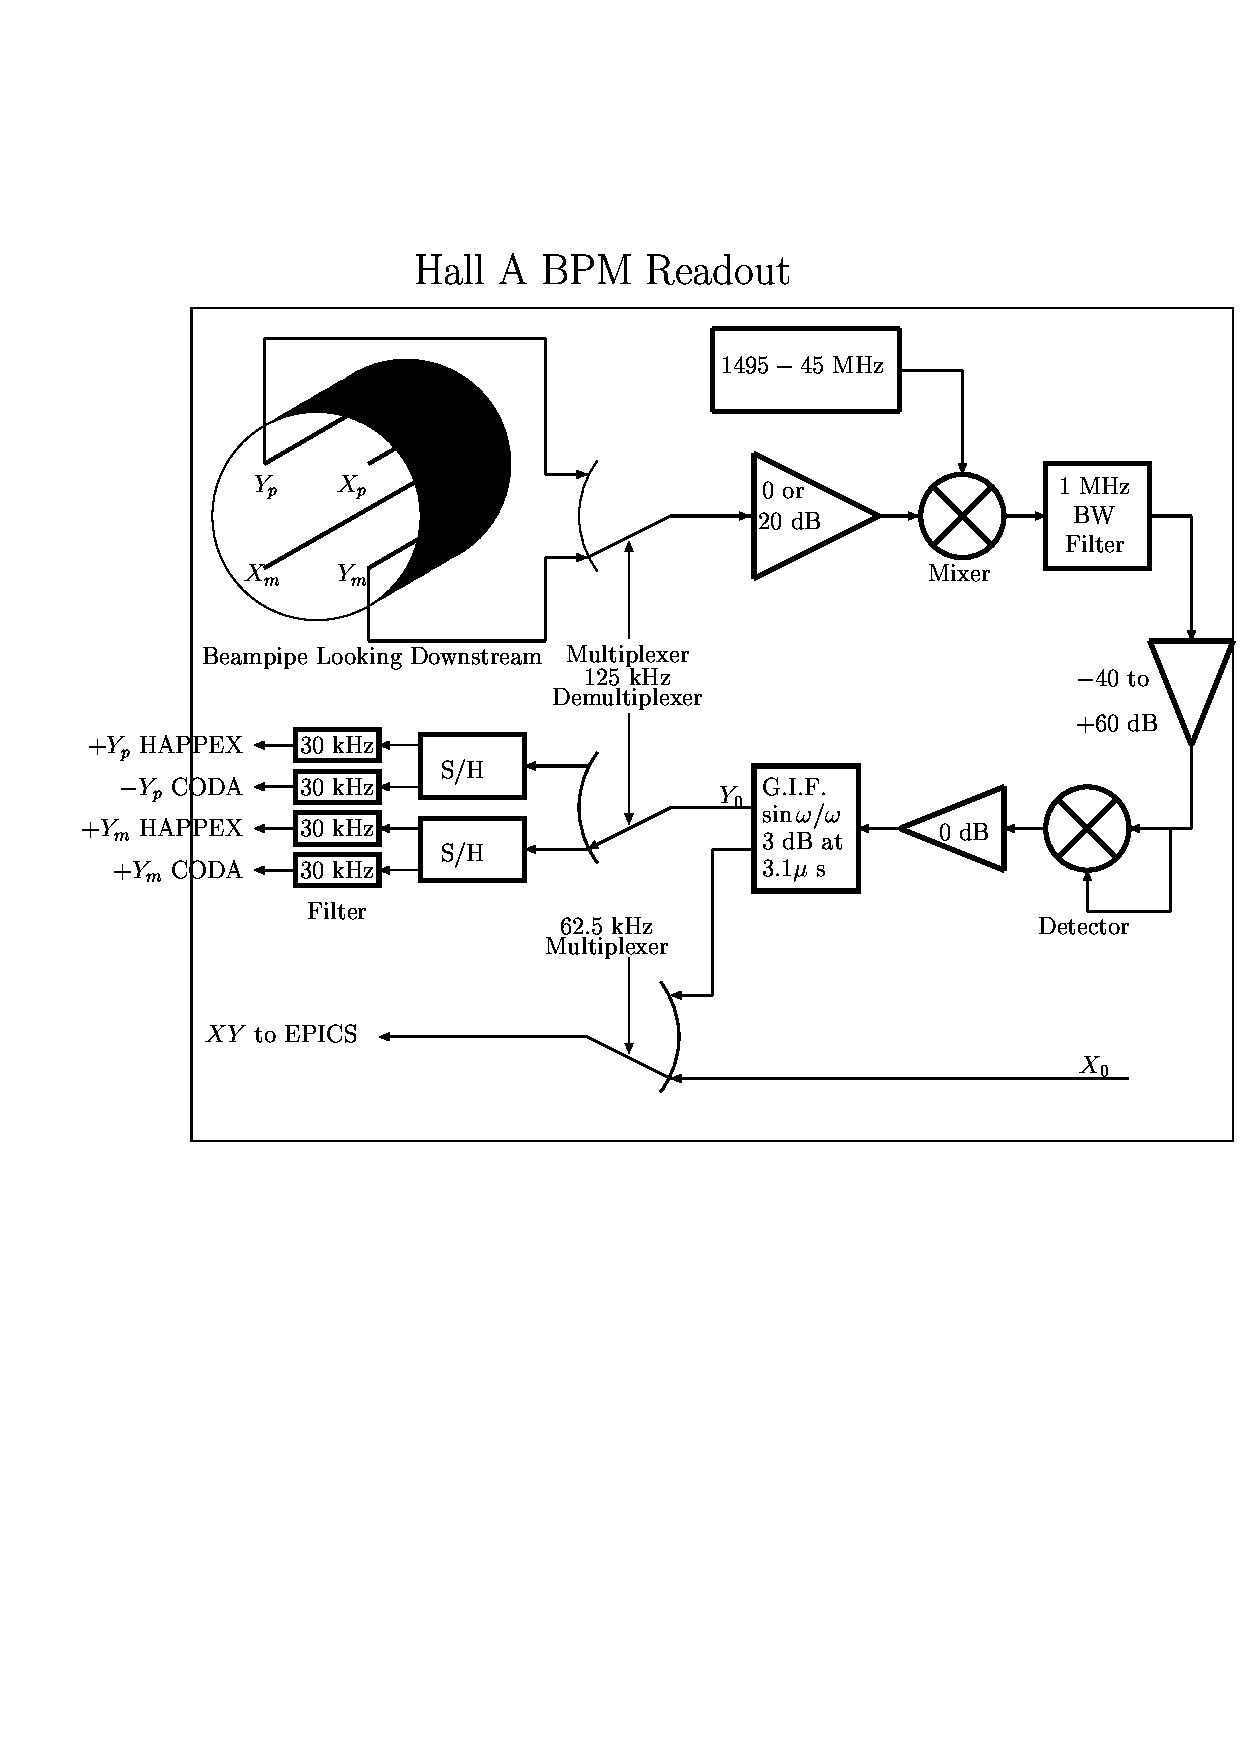
\includegraphics[angle=0,width=15cm]{BPM_fig}
{\linespread{1.}
\caption[Beamline: BPM Readout Electronics]{Schematic of the BPM readout
electronics}
\label{fig:bpmel}}
\end{center}
\end{figure}
}

\infolevone{
1. The averaged position over 0.3 seconds is logged into the EPICS~\cite{EPICSwww} database (1 
Hz updating frequency) and injected into the datastream every 3-4 seconds, 
unsynchronized but with an reference timestamp. From these values we can 
consider that we know the average position of the beam calculated in the EPICS 
coordinate system which is left handed.

2. Approximately once a shift (or more often if requested by the experimenters) 
a B-scope procedure ~\cite{bi:TP} can be performed using the same EPICS electronics 
which then gives the peak-to-peak variation of the beam.

3. Event-by-event information from the BPMs are recorded in the CODA datastream
from each of the 8 BPM antennas (2x4) from which the position of the beam can be 
reconstructed. However, these raw values belong to a parallel electronics chain 
whose constants have to be retrieved by calibrations to the EPICS or scanner 
data. 

\subsection{Beam Exit Channel}

After the target vacuum chamber, which was built by
the University of Virginia, there is an exit beam pipe which 
transfers the scattered beam onto the dump tunnel under vacuum. This exit beam 
pipe is made of a thin walled aluminum spiral corrugated pipe of welded 
construction. The largest diameter is 36 inches with a 0.164 inches wall 
thickness and the smallest diameter is 6 inches with a 0.042 inches wall 
thickness. The whole assembly is rather light (approximately 800 kg) and is 
supported by H shaped adjustable stands. To prevent possible linear collapse 
of the larger diameter sections under vacuum load, four aluminum channels of 
total cross-sectional area of 3'' are welded to its side. A vacuum of 
10$^{-5}$ Torr is maintained with a turbomolecular pump. The exit face of this 
pipe has a 12'' port and is connected to the diffuser with a Beryllium 
window.

}

\infolevone{
\section{ Machine/Beamline protection system}
\label{sec:beam-fsd}

The MPS~\cite{MPScebaf} system is composed of the Fast Shutdown System (FSD), Beam Loss 
Monitor (BLM), and gun control system.

The FSD system is a network of permissive signals which terminate at the 
electron gun and chopper 1. The permissive to the gun and chopper
1 may be inhibited by any device connected to an FSD mode. Devices connected to the 
FSD system include vacuum valves, RF systems, Beam loss systems, beam current 
monitors, beam dumps, and particular to Hall A, the target motion mechanism 
and the raster (value and derivative).

The gun control system includes software program which monitors beam 
operating conditions and the state of the FSD and BLM systems. the program 
will warn the operators if a potential for beam damage exists. Potential for 
damage exists when running high average current beam, when FSD nodes are 
masked and when the beam power approaches the operating envelope limits for a 
specific beam dump.
}

\begin{safetyen}{0}{0}
\infolevone{\section{Safety Information}}
%
% Information for the ESAD
%

The beamline in the Hall provides the interface between the CEBAF accelerator
and the experimental hall.   All work on the beamline must be coordinated 
with both physics division and accelerator division; in order to ensure
safe and reliable transport of the electron beam to the dump.

\subsection{Hazards}

Along the beamline these various hazards can be found.  These include
radiation areas, vacuum windows, high voltage, and magnetic fields.

\subsection{Mitigations}

All magnets (dipoles, quadrupoles, sextupoles, beam correctors) and beam 
diagnostic devices (BPMs, scanners, Beam Loss Monitor, viewers) necessary for 
the transport of the beam are controlled by Machine Control Center (MCC) 
through EPICS~\cite{EPICSwww}, except for special elements which are addressed in the 
subsequent sections. The detailed safety operational procedures for the Hall 
A beamline should be essentially the same as the one for the CEBAF machine 
and beamline.\\ 
  
\noindent{}Personnel who need to work near or around the beamline should keep in mind the potential hazards:
\begin{itemize}
  \item Radiation ``Hot Spots'' - marked by ARM or RadCon personnel,
  \item Vacuum in the beam line tubes and other vessels,
  \item Thin windowed vacuum enclosures (e.g. the scattering chamber),
  \item Electric power hazards in vicinity of the magnets,
  \item Magnetic field hazards in vicinity of the magnets, and
  \item Conventional hazards (fall hazard, crane hazard etc.).
\end{itemize}

These hazards are noted by signs and the most hazardous 
areas along the beamline
are roped off to restrict access when operational.   
In particular, the scattering chamber, with it's large
volume and thin windows requires hearing protection once it has been evacuated.   
Signs are posted by RadCon for any hot spots along the beamline and
RadCon must be notified before work is done in a posted area.

Some magnets, as the M{\o}ller spectrometer elements, are covered with plastic
sheets for electric safety. Any access to these magnets requires
the ``Lock and Tag'' procedure~\cite{EHScebaf} and the appropriate training,
including the equipment-specific one. \\

\noindent{}Additional safety information is available in the following documents:
\begin{list}{--}{\setlength{\itemsep}{-0.15cm}}
  \item EH\&S Manual~\cite{EHScebaf};
  \item PSS Description Document~\cite{PSScebaf}
  \item Accelerator Operations Directive~\cite{AODcebaf};
\end{list}

\subsection{Responsible Personnel}

Since the beamline requires both accelerator and physics personnel to maintain
and operate and it is very important that both groups stay in contact that any 
work on the Hall A beamline is coordinated.

\begin{namestab}{tab:beam:personnel_beam}{Beam line: authorized personnel}{%
   Beamline physics division and accelerator division points-of-contact.}
  \namestabheader{Hall A Physicists}
  \DouglasHiginbotham{\em 1st Contact}
  \RobertMichaels{\em 2nd Contact}
  \namestabheader{Liaisons from Accelerator Division}
  \HariAreti{..to Physics}
  \YvesRoblin{..to Hall-A}
\end{namestab}
\end{safetyen}

